\section{Adaptive Sampling Strategies}
Performing UQ and Dynamic PRA can be
challenging from a computational point of view. The \textit{Forward}
sampling strategies reported in the previous Section can lead to a large number of
unnecessary evaluations of the physical model leading to an unacceptable resource expenses (CPU time).
In addition, the \textit{Forward} methodologies are not designed to leverage the information
content that is extractable from the simulations already concluded.

To overcome these limitations, in RAVEN several adaptive algorithms are available:
\begin{enumerate}
  \item \textit{Limit Surface Search}
  \item \textit{Adaptive Dynamic Event Tree}
  \item \textit{Adaptive Hybrid Dynamic Event Tree}
  \item \textit{Adaptive Sparse Grid}
  \item \textit{Adaptive Sobol Decomposition}.
\end{enumerate}
In this Section, we will only show how to use the first algorithm.

%%%%%%%%%%%%%%%%
\subsection{Limit Surface Search sampling through RAVEN}
\label{sub:LSsamplingExample}
The goal of this Section is to learn how to:
 \begin{enumerate}
   \item Set up a LS Search sampling for efficiently perturb a driven code
   \item Use the LS Integral Post-processor for computing the probability of failure of the system subject to the same
   ``goal'' function
   \item Plot the obtained LS.
\end{enumerate}
In order to accomplish these tasks, the following RAVEN \textbf{Entities} (XML blocks in the input files) are defined:
\begin{enumerate}
   \item \textbf{\textit{RunInfo}}:
     \xmlExample[arg,extension,pauseAtEnd,overwrite]{framework/user_guide/AdaptiveSamplingStrategies/adaptiveSamplingLSsearch.xml}{RunInfo}
   As shown in Section~\ref{sub:EntitiesAndFlow}, the \textit{RunInfo} \textbf{Entity} is intended to set up the analysis
   that the user wants to perform. In this specific case, three steps (\xmlNode{Sequence}) are  sequentially run
   using eight processors (\xmlNode{batchSize}).
   \item \textbf{\textit{Files}}:
     \xmlExample[arg,extension,pauseAtEnd,overwrite]{framework/user_guide/AdaptiveSamplingStrategies/adaptiveSamplingLSsearch.xml}{Files}
   Since the driven code uses a single input file, in this Section the original input is placed. As detailed in the user manual
   the attribute  \xmlAttr{name} represents the alias that is going to be
   used in all the other input blocks in order to refer to this file.
   \\In addition the output file used in \xmlNode{Sequence}
   \textit{computeLSintegral} is here inputted.
   \item \textbf{\textit{Models}}:
     \xmlExample[arg,extension,pauseAtEnd,overwrite]{framework/user_guide/AdaptiveSamplingStrategies/adaptiveSamplingLSsearch.xml}{Models}
 As mentioned above, the goal of this example is the employment of
 an efficient sampling strategy, having as goal the determination of the
 failure of a system.

 In addition to the previously explained Code
 model,
 the ROM of type \textit{SciKitLearn} is here specified. The ROM will be
 used in the adaptive sampling strategy \textit{LimitSurfaceSearch} in
 order to accelerate the convergence of the method. As it can be seen,
 a nearest neighbor classifier is used, targeting only two uncertainties
 $sigma-A and decay-A$.
 \\ For the computation of the probability of failure (see the following), a
 Post-Processor (PP) of type \textit{LimitSurfaceIntegral} is here
 specified.This PP performs an integral of the LS
 generated by the adaptive sampling technique.
   \item \textbf{\textit{Distributions}}:
     \xmlExample{framework/user_guide/AdaptiveSamplingStrategies/adaptiveSamplingLSsearch.xml}{Distributions}
  In the Distributions XML Section, the stochastic model for the
  uncertainties  treated by the LS search sampling are reported. In
  this case two distributions are defined:
  \begin{itemize}
    \item $sigmaA \sim \mathbb{U}(0,1000)$, used to model the uncertainty
    associated with  the Model \textit{sigma-A}
    \item  $decayConstantA \sim \mathbb{U}(1e-8,1e-7)$,  used to
    model the uncertainty
    associated with  the Model \textit{decay-A}.
  \end{itemize}
   \item \textbf{\textit{Samplers}}:
     \xmlExample[arg,extension,pauseAtEnd,overwrite]{framework/user_guide/AdaptiveSamplingStrategies/adaptiveSamplingLSsearch.xml}{Samplers}
  In order to employ the LS search sampling strategy, a
  \xmlNode{LimitSurfaceSearch} node needs to be inputted.
  As it can be
  seen from above, each variable is associated to a different distribution
  defined in the  \xmlNode{Distributions} block.
  In addition, the \textit{AccelerationROM}  \xmlNode{ROM} is inputted.
  As already mentioned, this ROM (of type classifier) is used to
  accelerate the convergence of the LS Search method.
  In addition, the goal function \textit{goalFunction}  and the
  \textit{samples} are here reported.
  \\For this example, a convergence criterion of $1.0e-5$ is set. To reach such a confidence with a Monte-Carlo, millions of
  samples would be needed.
   \item \textbf{\textit{Functions}}:
     \xmlExample[arg,extension,pauseAtEnd,overwrite]{framework/user_guide/AdaptiveSamplingStrategies/adaptiveSamplingLSsearch.xml}{Functions}
 As already mentioned, the LS search sampling strategy uses
 a goal function in order to identify the regions of the uncertain space
 that are more informative. The \textit{goalFunction} used for this
 example is reported below. As it can be seen, if the final response $A$
 is $<=$ of $0.3$ , the system is considered to be in a ``safe'' condition.
\begin{lstlisting}[language=python]
def __residuumSign(self):
  returnValue = 1.0
  if self.A  <= 0.3:
    returnValue = -1.0
  return returnValue
\end{lstlisting}

   \item \textbf{\textit{DataObjects}}:
     \xmlExample[arg,extension,pauseAtEnd,overwrite]{framework/user_guide/AdaptiveSamplingStrategies/adaptiveSamplingLSsearch.xml}{DataObjects}
      In this block, three \textit{DataObjects} are defined: 1) PointSet
      named ``samples'' used to collect the final outcomes of the code, 2)
      HistorySet named ``histories'' in which the full time responses of the
      variables $A,B,C,D$ are going to be stored, 3) PointSet named
      ``limitSurface'' used  to export the LS location (in the uncertain space) during the employment of the sampling strategy.
   \item \textbf{\textit{OutStreams}}:
     \xmlExample[arg,extension,pauseAtEnd,overwrite]{framework/user_guide/AdaptiveSamplingStrategies/adaptiveSamplingLSsearch.xml}{OutStreams}
     Several out streams are included in this workflow, two for printing and three for plotting:
     \begin{itemize}
       \item ``samples'', which writes the validation sample contents of the \xmlString{samples} PointSet DataObject to a CSV file,
       \item ``histories'', which writes the sampling contents of the \xmlString{histories} HistorySet DataObject to a
         set of connected CSV files,
       \item ``historyPlot'', which plots the evolution of the samples taken,
       \item ``limitSurfacePlot'', which plots the limit surface discovered by the PostProcessor,
       \item ``samplesPlot3D'', which plots the final state of the samples taken against the figures of merit.
     \end{itemize}
     The plots demonstrate how visualization of three-dimensional data, time-dependent data, and limit
     surfaces can be realized using RAVEN.
 %%%%%%%%%%%%%%%%%%%%%%%%%%%%%%%%%%%%%%%%%%%%%%%%%%%%%%%%%%
 %%%%%%%%%%%%%%%%%%%%%%%%%%%%%%%%%%%%%%%%%%%%%%%%%%%%%%%%%%
 %figure samples
 \begin{figure}[h!]
  \centering
  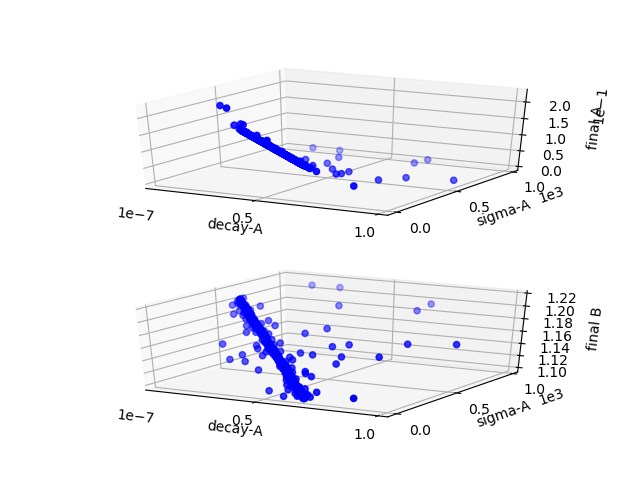
\includegraphics[scale=0.7]{../../tests/framework/user_guide/AdaptiveSamplingStrategies/gold/LSsearch/1-samplesPlot3D_scatter-scatter.png}
  \caption{Plot of the samples generated by the LS search sampling for variables $A,B$.}
  \label{fig:LS_pointsets}
 \end{figure}
 %%%%%%%%%%%%%%%%%%%%%%%%%%%%%%%%%%%%%%%%%%%%%%%%%%%%%%%%%%
 %%%%%%%%%%%%%%%%%%%%%%%%%%%%%%%%%%%%%%%%%%%%%%%%%%%%%%%%%%
   \item \textbf{\textit{Steps}}:
     \xmlExample[arg,extension,pauseAtEnd,overwrite]{framework/user_guide/AdaptiveSamplingStrategies/adaptiveSamplingLSsearch.xml}{Steps}
  %%%%%%%%%%%%%%%%%%%%%%%%%%%%%%%%%%%%%%%%%%%%%%%%%%%%%%%%%%
 %figure samples
 \begin{figure}[h!]
  \centering
  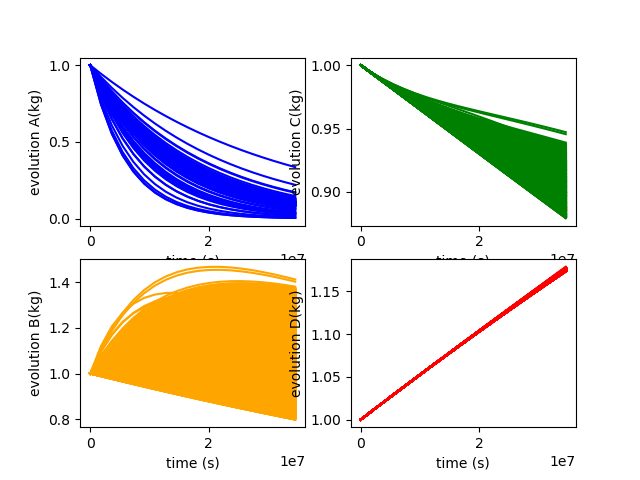
\includegraphics[scale=0.7]{../../tests/framework/user_guide/AdaptiveSamplingStrategies/gold/LSsearch/1-historyPlot_line-line-line-line.png}
  \caption{Plot of the histories generated by the LS search method for variables $A,B,C,D$.}
  \label{fig:LS_histories}
 \end{figure}
 %%%%%%%%%%%%%%%%%%%%%%%%%%%%%%%%%%%%%%%%%%%%%%%%%%%%%%%%%%
   Finally, all the previously defined \textbf{Entities} can be combined in
   the \xmlNode{Steps} block. As inferable,
   three \xmlNode{Steps} have been inputted:
   \begin{itemize}
     \item \xmlNode{MultiRun} named ``sample'', used to run the multiple
     instances of the driven code and
     collect the outputs in the two \textit{DataObjects}. As it can be
     seen, the \xmlNode{Sampler} is inputted to communicate to the
     \textit{Step} that the driven code needs to
     be perturbed through the LS search sampling strategy;
     \item \xmlNode{PostProcess} named ``computeLSintegral'', used to
     compute the probability of failure of the system based on the LS generated employing the LS search strategy. This
     probability is computed integrating the LS with a Monte-Carlo
     method.
     \item  \xmlNode{IOStep} named ``writeHistories'', used to 1) export
     the ``histories'' and ``samples''  \textit{DataObjects}
     \textbf{Entity} in a CSV file and 2) plot the data and the Limit Surface
     in  PNG files and on the screen.
   \end{itemize}
\end{enumerate}
 Figure~\ref{fig:LS_histories}
 shows the evolution of the outputs $A,B,C,D$ under uncertainties.
 Figure~\ref{fig:LS_pointsets} shows the final responses  of $A and B$
 of the sampling employed using the driven code.
 Figure~\ref{fig:LSplot}  shows the limit surface for this particular
 example. Only $367$ samples were needed in order to reach the full
 convergence.
 \\The integration of the LS determines a probability of failure of
 $~3.45e-2$.
  %%%%%%%%%%%%%%%%%%%%%%%%%%%%%%%%%%%%%%%%%%%%%%%%%%%%%%%%%%
 %figure samples
 \begin{figure}[h!]
  \centering
  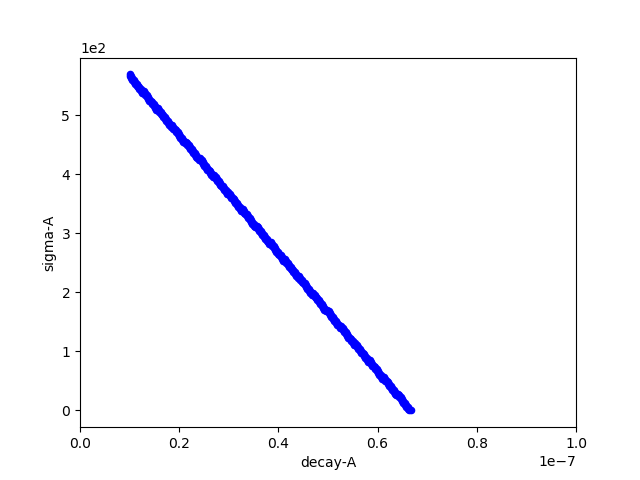
\includegraphics[scale=0.7]{../../tests/framework/user_guide/AdaptiveSamplingStrategies/gold/LSsearch/1-limitSurfacePlot_scatter.png}
  \caption{Limit Surface generated by the LS search method.}
  \label{fig:LSplot}
 \end{figure}
 %%%%%%%%%%%%%%%%%%%%%%%%%%%%%%%%%%%%%%%%%%%%%%%%%%%%%%%%%%








